\documentclass[tikz,border=5pt]{standalone}
\usepackage{amsmath,amssymb}
\usetikzlibrary{arrows.meta}

% \sets{<prefix>}{<x-shift>}{<label A>}{<label B>}
% Draws the two rounded boxes with elements 1,2,3 and x,y,z.
% Nodes are named <prefix>a1..a3 and <prefix>b1..b3.
\newcommand{\sets}[4]{%
  \begin{scope}[shift={(#2,0)}]
    \draw[thick, fill=blue!5!white, rounded corners=15pt] (-1.5,-2) rectangle (-0.2,2);
    \draw[thick, fill=red!5!white,  rounded corners=15pt] ( 0.8,-2) rectangle ( 2.1,2);
    \node at (-1.00,2.35) {#3};
    \node at ( 1.80,2.35) {#4};
    \node (#1a1) at (-0.85, 1) {$1$};
    \node (#1a2) at (-0.85, 0) {$2$};
    \node (#1a3) at (-0.85,-1) {$3$};
    \node (#1b1) at ( 1.45, 1) {$x$};
    \node (#1b2) at ( 1.45, 0) {$y$};
    \node (#1b3) at ( 1.45,-1) {$z$};
  \end{scope}%
}

\begin{document}
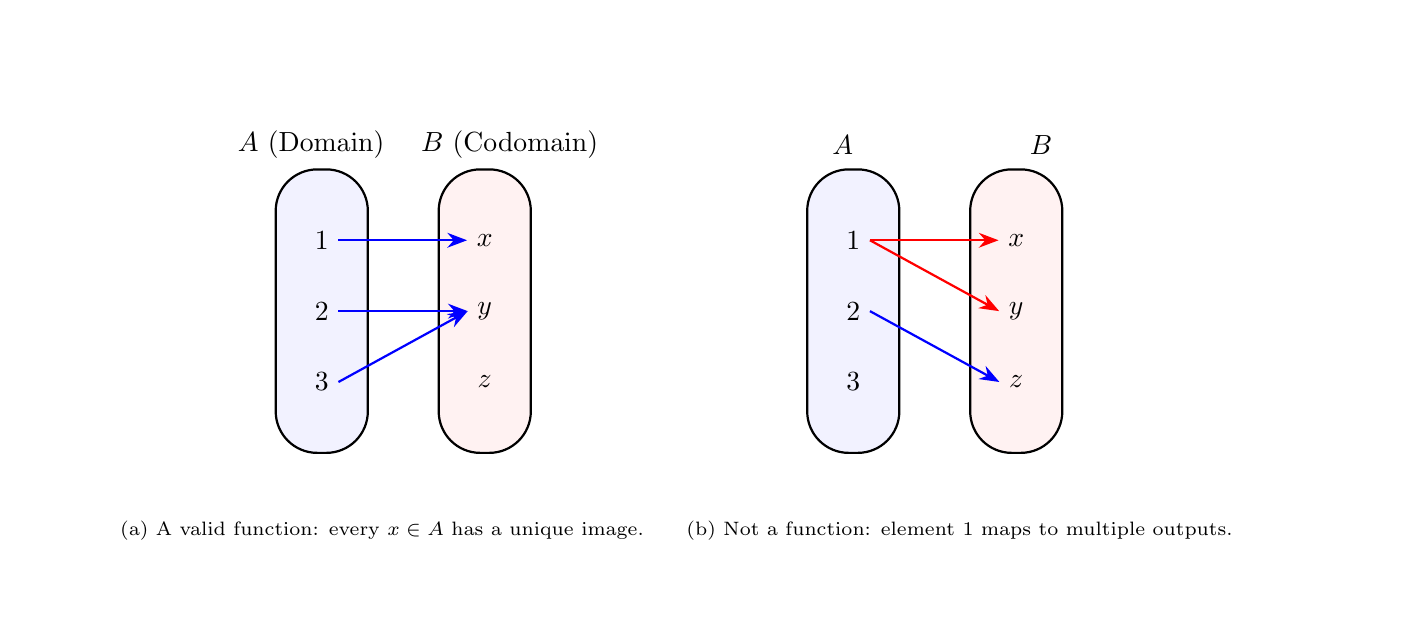
\begin{tikzpicture}[scale=0.9, every node/.style={font=\normalsize},
  arr/.style={-{Stealth[length=2.5mm]}, thick},
  cap/.style={text width=5cm, align=center, font=\tiny}]

  \fill[white] (-5,-4) rectangle (14,4);

  % ---------- Panel (a): valid function ----------
  \sets{f}{0.0}{$A$ (Domain)}{$B$ (Codomain)}
  \draw[arr, blue] (fa1.east) -- (fb1.west);
  \draw[arr, blue] (fa2.east) -- (fb2.west);
  \draw[arr, blue] (fa3.east) -- (fb2.west);
  \node at (0.0,-3.1)
    {\scriptsize{(a) A valid function: every $x \in A$ has a unique image.}};

  % ---------- Panel (b): not a function ----------
  \sets{g}{7.5}{$A$}{$B$}
  \draw[arr, red]  (ga1.east) -- (gb1.west);
  \draw[arr, red]  (ga1.east) -- (gb2.west);
  \draw[arr, blue] (ga2.east) -- (gb3.west);
  \node at (8.15,-3.1)
    {\scriptsize{(b) Not a function: element $1$ maps to multiple outputs.}};

\end{tikzpicture}
\end{document}






% \documentclass{standalone}
% \usepackage[utf8]{inputenc}
% \usepackage{tikz}
% \usepackage{subcaption}
% \usepackage{amsmath,amssymb}
% \usepackage{geometry}
% % \geometry{a4paper, margin=1in}
% 
% \begin{document}
% 
% % \section*{Session 1 Visualizations}
% 
% % --- FIGURE 1: Functions vs Relations ---
% \begin{figure}[htbp]
% \centering
% \begin{subfigure}[b]{0.48\textwidth}
% \centering
% \begin{tikzpicture}[scale=0.9]
%     % Sets A and B
%     \draw[thick, fill=blue!5!white, rounded corners=15pt] (-1.5,-2) rectangle (-0.2,2);
%     \draw[thick, fill=red!5!white, rounded corners=15pt] (0.8,-2) rectangle (2.1,2);
%     \node at (-0.85, 2.3) {$A$ (Domain)};
%     \node at (1.45, 2.3) {$B$ (Codomain)};
%     
%     % Elements of A
%     \node (a1) at (-0.85, 1) {$1$};
%     \node (a2) at (-0.85, 0) {$2$};
%     \node (a3) at (-0.85,-1) {$3$};
%     
%     % Elements of B
%     \node (b1) at (1.45, 1) {$x$};
%     \node (b2) at (1.45, 0) {$y$};
%     \node (b3) at (1.45,-1) {$z$};
%     
%     % Arrows (Valid function)
%     \draw[->, thick, >=stealth, blue] (a1) -- (b1);
%     \draw[->, thick, >=stealth, blue] (a2) -- (b2);
%     \draw[->, thick, >=stealth, blue] (a3) -- (b2);
% \end{tikzpicture}
% \caption{A valid function: every $x \in A$ has a unique image.}
% \end{subfigure}
% \hfill
% \begin{subfigure}[b]{0.48\textwidth}
% \centering
% \begin{tikzpicture}[scale=0.9]
%     % Sets A and B
%     \draw[thick, fill=blue!5!white, rounded corners=15pt] (-1.5,-2) rectangle (-0.2,2);
%     \draw[thick, fill=red!5!white, rounded corners=15pt] (0.8,-2) rectangle (2.1,2);
%     \node at (-0.85, 2.3) {$A$};
%     \node at (1.45, 2.3) {$B$};
%     
%     % Elements of A
%     \node (a1) at (-0.85, 1) {$1$};
%     \node (a2) at (-0.85, 0) {$2$};
%     \node (a3) at (-0.85,-1) {$3$};
%     
%     % Elements of B
%     \node (b1) at (1.45, 1) {$x$};
%     \node (b2) at (1.45, 0) {$y$};
%     \node (b3) at (1.45,-1) {$z$};
%     
%     % Arrows (Violation: multiple outputs for element 1)
%     \draw[->, thick, >=stealth, red] (a1.east) -- (b1.west);
%     \draw[->, thick, >=stealth, red] (a1.east) -- (b2.west);
%     \draw[->, thick, >=stealth, blue] (a2) -- (b3);
% \end{tikzpicture}
% \caption{Not a function: element $1$ maps to multiple outputs.}
% \end{subfigure}
% \caption{Comparison between a function and a general relation.}
% \end{figure}
% 
% 
% \end{document}
